\documentclass[11pt, a4paper]{article}
\usepackage[utf8]{inputenc}
\usepackage[T1]{fontenc}
\usepackage[french]{babel}
\usepackage{geometry}
\geometry{top=2cm, bottom=2.5cm, left=2.5cm, right=2.5cm}

\usepackage{graphicx}
\usepackage{titlesec}
\usepackage{enumitem}
\usepackage{xcolor}
\usepackage{float}
% Couleurs

% Charte graphique - couleurs Esaip
\usepackage[many]{tcolorbox}
\definecolor{EsaipDarkBlue}{HTML}{242756}
\definecolor{EsaipBlue}{HTML}{3878BD}
\definecolor{EsaipGreen}{HTML}{3AAE70}
\definecolor{EsaipRed}{HTML}{E83C45}
\definecolor{EsaipOrange}{HTML}{F6A02A}

\usepackage{hyperref}
\hypersetup{colorlinks=true, linkcolor=blue, urlcolor=blue}

% ---- Style des sections ----
\titleformat{\section}{\large\bfseries\scshape}{}{0em}{}[\titlerule]
\titlespacing*{\section}{0pt}{12pt}{6pt}
\titleformat{\subsection}{\bfseries}{}{0em}{}
\titlespacing*{\subsection}{0pt}{8pt}{4pt}

% ---- Commandes personnalisées pour remplir facilement le titre ----
\newcommand{\projecttitle}[1]{\def\theprojecttitle{#1}}
\newcommand{\groupmembers}[1]{\def\thegroupmemberlist{#1}}
% Initialisation par défaut (évite les erreurs si non défini)
\def\thegroupmemberlist{\emph{(Liste des membres non définie)}}

\newcommand{\coursename}[1]{\def\thecoursename{#1}}
\newcommand{\referent}[1]{\def\referent{#1}}

%=====================================================================
% --- Paramètres à modifier par chaque groupe ---
\projecttitle{L'aérodynamisme d'une F1}
\groupmembers{Mathis CORCIA \\ Paul RANDON}
\coursename{Démarche Scientifique}
\referent{Nicolas Michel}

%=====================================================================

\begin{document}

% ====================
% PAGE DE TITRE
% ====================
\begin{titlepage}

% Contenu
    \centering
    {\LARGE \bfseries Journal de bord réflexif}\\%[0.25cm]
    {\Large Cahier de laboratoire de la Situation d'Apprentissage et d'Évaluation}

    \hrulefill\\[1cm]
    
    {\large \bfseries Projet Scientifique :} \par
    {\color{EsaipBlue}\textbf{\Huge \theprojecttitle}} \par\vspace{1.5cm}
    \begin{minipage}[t]{0.9\textwidth}
        \centering
        \large
        Situation d'apprentissage et d'évaluation :\par
        \textbf{\thecoursename} \\[0.5cm]
    \end{minipage}
    \begin{figure}[H]
    \centering
    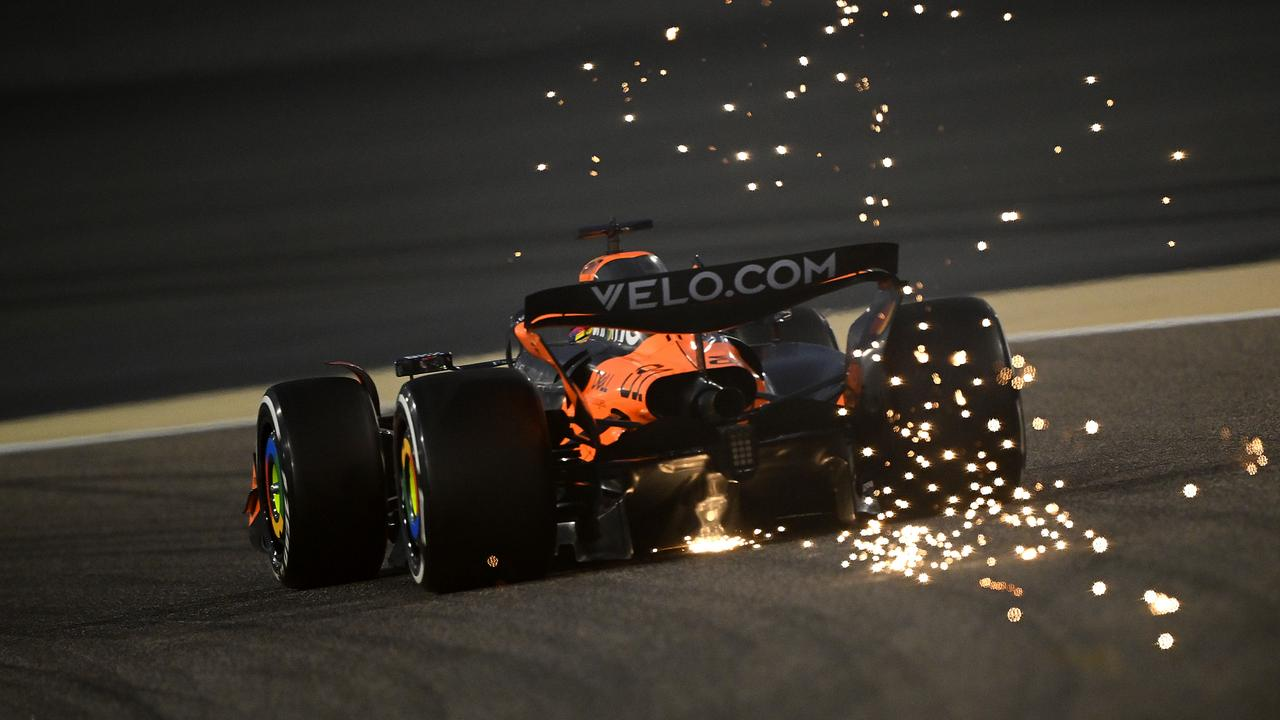
\includegraphics{Images/F1.png}
    \end{figure} 
    \vfill
    \textbf{Groupe :} \\ % Libellé sur sa propre ligne
    % Affichage de la liste stockée, chaque élément dans un tableau
        \begin{tabular}[t]{@{}l@{}} 
            \thegroupmemberlist 
            
        \end{tabular} \\[0.8cm] % [t] pour alignement vertical en haut
    \textbf{Enseignant·e référent·e :} \referent \\[2cm]
    % Logo
     
\includegraphics[width=0.3\textwidth]{Images/Logo_Esaip_Couleur.png}
    %\vfill
    
    {\large 2025-2026}
\end{titlepage}

% ====================
% INSTRUCTIONS
% ====================
\section*{Instructions d'utilisation}
\noindent Ce journal est la \textbf{trace écrite de votre raisonnement scientifique}. Complétez-le régulièrement, de manière individuelle ou collective, pour documenter votre démarche, pas seulement vos actions.
\begin{itemize}[leftmargin=*]
    \item[$\bullet$] \textbf{Objectif :} analyser vos choix, difficultés, réussites et apprentissages à chaque étape.
    \item[$\bullet$] \textbf{Évaluation :} la qualité de votre réflexion nourrira l'évaluation de la compétence \emph{"Réflexivité \& Auto-évaluation"}.
    \item[$\bullet$] \textbf{Conseil :} soyez honnêtes et détaillés. Une difficulté bien analysée a plus de valeur qu'un succès simplement énoncé.
\end{itemize}

% ====================
% Séance de lancement
% ====================
\section{Séance 1 : Lancement \& émergence de la problématique}

\medskip

\textbf{Date : 18/02/2026}

\medskip

\subsection{Notre question de recherche initiale}
\noindent
\framebox[\textwidth][l]{\parbox{0.95\textwidth}{\vspace{0.9cm} % Boîte pour la question
    \textit{Comment les variations de densité de l'air (altitude à Mexico vs niveau de la mer) affectent-elles la sensibilité d'une F1 ?} \par
    \vspace{0.9cm}
}}

\subsection{Notre cheminement intellectuel}
\begin{enumerate}
    \item \textbf{Observations/Idées de départ : }
    \textbf{ Les conditions doivent varier de manière assez sensible ; cependant,} 
    
    \bigskip
    
    \item \textbf{Pourquoi cette question nous intéresse-t-elle ?} 
    
    \bigskip
    
    \item \textbf{Hypothèse(s) formulée(s) :} 
    
    Nous pensons que moins l'air est dense, moins l'aérodynamisme est important 

    \medskip
    
    parce qu'il y a moins de frottement avec l'air

    \bigskip
    

\end{enumerate}

\subsection{Ressenti et prospective}
\begin{itemize}
    \item[$\bullet$] \textbf{Nos premières inquiétudes / défis anticipés :}
    \item[$\bullet$] \textbf{Point(s) à clarifier avec l'enseignant·e :}
\end{itemize}

% ====================
% Conception du protocole
% ====================
\newpage
\section{Étape 2 : Conception du protocole expérimental}

\medskip

\textbf{Date :} 

\medskip

\subsection{De la question au plan d'expérience}

\textbf{Schéma ou description clé du montage :} \\[0.5cm]
\framebox[\textwidth][l]{\parbox{0.95\textwidth}{\vspace{4cm}}} % Espace pour un schéma

\subsection{Variables et paramètres identifiées}
\begin{itemize}
    \item[$\bullet$] \textbf{Variable indépendante (celle que l'on modifie) :}
    \item[$\bullet$] \textbf{Variable dépendante (celle que l'on mesure) :}
    \item[$\bullet$] \textbf{Paramètres à contrôler (constantes) :}
\end{itemize}

\subsection{Analyse réflexive de l'étape}
\begin{itemize}
    \item[$\bullet$] \textbf{Difficulté majeure rencontrée :}
    \item[$\bullet$] \textbf{Comment nous l'avons surmontée (ou tentative) :}
    \item[$\bullet$] \textbf{Modification apportée suite au feedback :}
\end{itemize}

\newpage
% ====================
% Expérimentation
% ====================
\section{Étape 3 : Réalisation expérimentale \& collecte des données}

\medskip

\textbf{Date(s) de manipulation :}

\medskip

\subsection{Déroulement et observations}
\begin{itemize}
    \item[$\bullet$] \textbf{Écart(s) par rapport au protocole prévu :}
    \item[$\bullet$] \textbf{Observation inattendue ou problème technique :}
    \item[$\bullet$] \textbf{Décision prise sur le moment et sa justification :}
\end{itemize}

\subsection{Rigueur et incertitudes}
\begin{itemize}
    \item[$\bullet$] \textbf{Mesures prises pour assurer la reproductibilité (ex: répétitions) :}
    \item[$\bullet$] \textbf{Sources d'erreur ou d'incertitude identifiées :}
\end{itemize}

\newpage
% ====================
% Analyse des résultats
% ====================
\section{Étape 4 : Analyse des données \& interprétation}

\medskip

\textbf{Date :}

\medskip

\subsection{Traitement des données}
\begin{itemize}
    \item[$\bullet$] \textbf{Outils/méthodes utilisés (tableur, régression, test statistique) :}
    \item[$\bullet$] \textbf{Figure ou tableau clé produit (joindre en annexe ou décrire) :}
    \item[$\bullet$] \textbf{Résultat numérique principal :}
\end{itemize}

\subsection{Interprétation critique}
\begin{itemize}
    \item[$\bullet$] \textbf{Comment nos résultats répondent-ils à la question initiale ?}
    \item[$\bullet$] \textbf{Sont-ils en accord avec notre hypothèse ? Si non, pourquoi ?}
    \item[$\bullet$] \textbf{Limite(s) principale(s) de notre étude qui pourraient affecter les résultats :}
\end{itemize}

\newpage
% ====================
% Communication et bilan
% ====================
\section{Étape 5 : Communication \& bilan final du projet}

\medskip

\textbf{Date de finalisation :} \hrulefill

\medskip

\subsection{Retour sur la démarche}
\begin{itemize}
    \item[$\bullet$] \textbf{Le point le plus difficile du projet a été :}
    \item[$\bullet$] \textbf{Le principal apprentissage méthodologique est :}
    \item[$\bullet$] \textbf{Si c'était à refaire, nous modifierions :}
\end{itemize}

\subsection{Projection}
\begin{itemize}
    \item[$\bullet$] \textbf{Question de recherche nouvelle qui émerge de ce travail :}
    \item[$\bullet$] \textbf{Comment les compétences développées ici seront utiles ailleurs :}
\end{itemize}

\end{document}
